% Made up for the tikra benchmark.
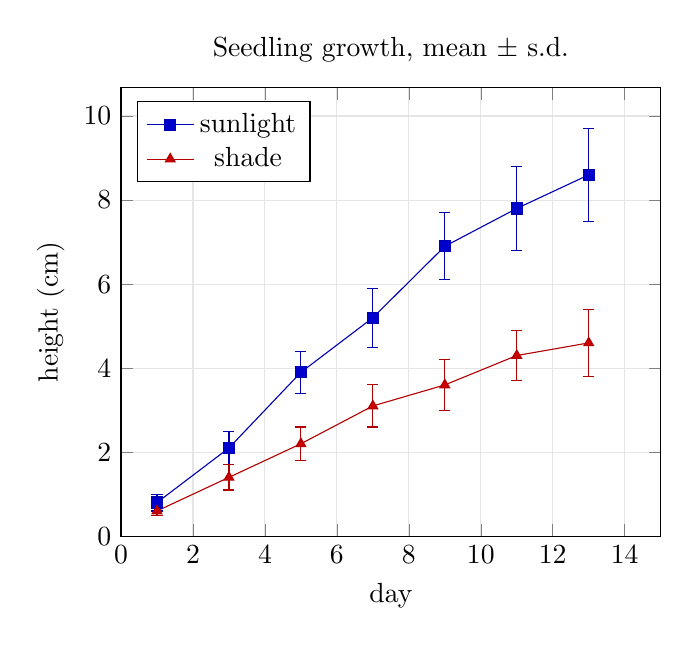
\begin{tikzpicture}
\begin{axis}[xlabel={day}, ylabel={height (cm)}, title={Seedling growth, mean $\pm$ s.d.},
    legend pos=north west, grid=major, grid style={gray!20}, xmin=0, xmax=15, ymin=0]
  \addplot+[mark=square*, blue!70!black, error bars/.cd, y dir=both, y explicit]
    coordinates {(1,0.8) +- (0,0.2) (3,2.1) +- (0,0.4) (5,3.9) +- (0,0.5) (7,5.2) +- (0,0.7)
      (9,6.9) +- (0,0.8) (11,7.8) +- (0,1.0) (13,8.6) +- (0,1.1)};
  \addplot+[mark=triangle*, red!70!black, error bars/.cd, y dir=both, y explicit]
    coordinates {(1,0.6) +- (0,0.1) (3,1.4) +- (0,0.3) (5,2.2) +- (0,0.4) (7,3.1) +- (0,0.5)
      (9,3.6) +- (0,0.6) (11,4.3) +- (0,0.6) (13,4.6) +- (0,0.8)};
  \legend{sunlight, shade}
\end{axis}
\end{tikzpicture}
